
%(BEGIN_QUESTION)
% Copyright 2006, Tony R. Kuphaldt, released under the Creative Commons Attribution License (v 1.0)
% This means you may do almost anything with this work of mine, so long as you give me proper credit

Describe all that is represented by this P\&ID:

$$\includegraphics[width=15.5cm]{i00219x01.eps}$$

\underbar{file i00219}
%(END_QUESTION)





%(BEGIN_ANSWER)

This is a pressure control system for an air compressor.  It uses two pressure switches, a high (``PSH'') and a low (``PSL''), sending on-off electrical signals to a logic control circuit (possibly a PLC).  The logic then turns the compressor motor on and off.

A rupture disk is provided at the receiver tank for high pressure relief, and a hand-operated ball valve provides blowdown control.

The ``PSHH'' bubble is a high-high pressure switch, activated only when the receiver tank pressure is above normal operating pressure.  It sends an on-off electrical signal to a high pressure alarm (``PAH'') indicator.

%(END_ANSWER)





%(BEGIN_NOTES)

Be sure to ask your students specifically what symbols represent all the things identified in the answer!

%INDEX% Process: air compressor and receiver tank
%INDEX% Switch, pressure: P&ID symbols

%(END_NOTES)


